\subsection{Implementasi Arsitektur \textit{Microservices} Menggunakan Komunikasi \textit{Event-Driven} Pada Aplikasi Pemesanan Tiket Acara (Jeeves)}

Tugas akhir ini membahas aplikasi pemesanan tiket acara dengan arsitektur \textit{microservice} dengan komunikasi \textit{event-driven}. Tujuan dari penelitian tersebut adalah membuat aplikasi \textit{ticketing} yang \textit{fault-tolerant} sehingga \textit{service} yang masih berjalan tetap dapat memenuhi aksi yang lain. Untuk itu, arsitektur \textit{microservice} diimplementasikan dengan cara \textit{loosely-coupled}. Untuk memenuhi hal itu, komunikasi \textit{event-driven} digunakan. Agar \textit{dependency} antar-\textit{service} berkurang, seluruh data yang diperlukan oleh sebuah \textit{service} diikutserkatan pada \textit{event} yang dikirim \parencite{microservicesEventDriven}.

\begin{figure}[ht]
    \centering
    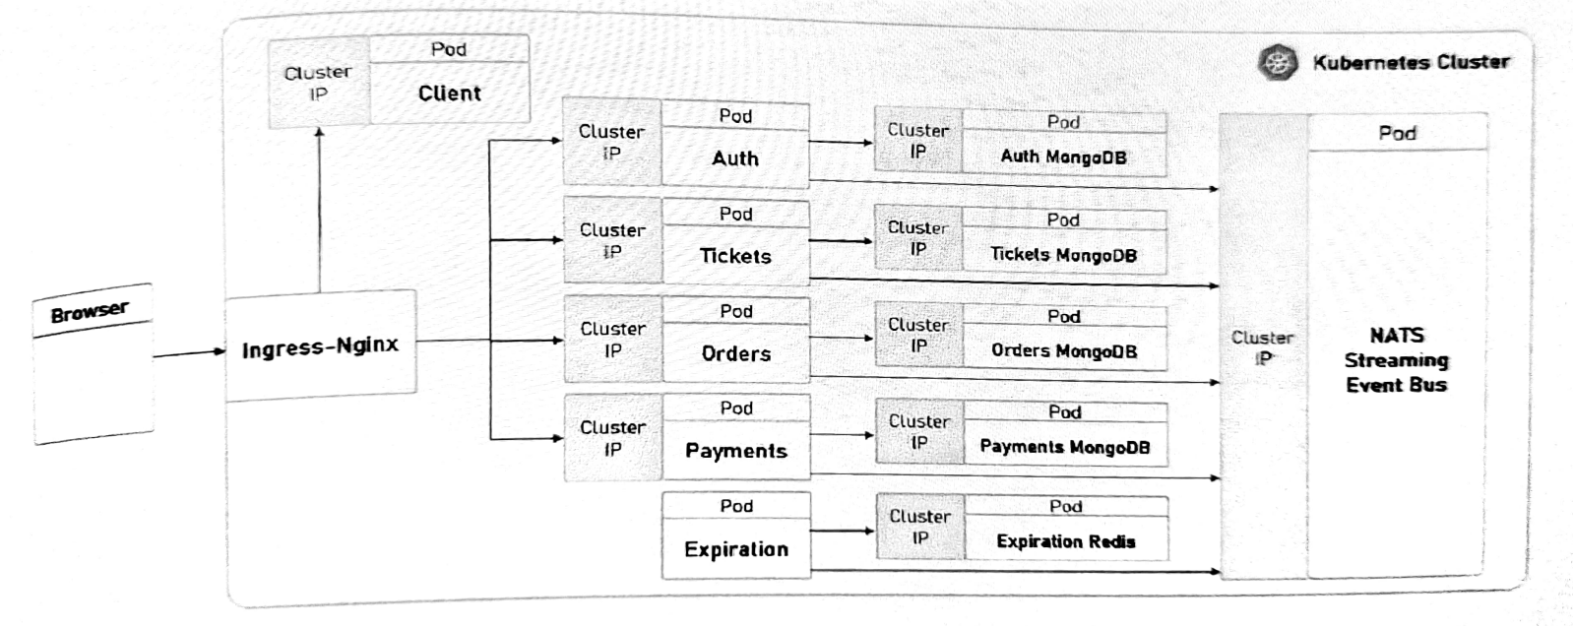
\includegraphics[width=1\textwidth]{resources/chapter-2/jeeves.png}
    \caption{\textit{Arsitektur Jeeves \parencite{microservicesEventDriven}}}
    \label{fig:jeeves-architecture}
\end{figure}

Penelitian ini mengimplementasikan fungsionalitas dasar seperti otentikasi pengguna, pembuatan tiket, reservasi tiket, dan pembayaran tiket. Terdapat lima \textit{microservices} yang dibuat, yaitu \textit{authentication service}, \textit{tickets microservice}, \textit{orders microservice}, \textit{payments microservice}, dan \textit{expiration microservice}. Setiap \textit{microservice} selain \textit{expiration microservice} memiliki basis data masing-masing menggunakan MongoDB. Hanya \textit{expiration microservice} yang menggunakan Redis. Selain itu, setiap komunikasi yang terjadi secara \textit{asynchronous} dilakukan melalui \textit{messaging platform} NATS. Untuk melakukan validasi otentikasi, sistem ini menggunakan JWT dengan \textit{shared secret} yang di-\textit{manage} oleh Kubernetes. Pendekatan ini memungkinkan \textit{service} independen terhadap \textit{authentication microservice} \parencite{microservicesEventDriven}.

Penelitian ini berhasil mengimplementasikan arsitektur aplikasi untuk pemesanan tiket acara yang \textit{fault-tolerant} dengan pendekatan \textit{microservices} dan \textit{event-driven architecture}. Meskipun begitu, penelitian ini tidak membahas dan menguji aspek \textit{scalability} dan \textit{elasticity} dari sistem ini.